\documentclass[]{article}
\usepackage[utf8]{inputenc}
\usepackage[slovak]{babel}
\usepackage[hidelinks]{hyperref}
\usepackage{graphicx}

\begin{document}

\begin{titlepage}
	\begin{center}
		\textsc{{\LARGE Vysoké učení technické v~Brně\\[0.3em]
				Fakulta informačních technologií}}\\
		\vspace{\stretch{0.382}}
		{\Huge \textbf{Simulačné štúdium}\\[0.5em]Spracovanie železa a oceli}
		\vspace{\stretch{0.618}}
	\end{center}

	{\noindent \large Lukáš Dekrét\\Dávid Bolvanský\hfill \today}
\end{titlepage}

\section{Úvod}
V~našej práci sme modelovali a simulovali\footnote{\url{https://www.fit.vutbr.cz/study/courses/IMS/public/prednasky/IMS.pdf}, strana 8} proces výroby oceľových rúr zo šrotu. Na základe modelu\footnote{\url{https://www.fit.vutbr.cz/study/courses/IMS/public/prednasky/IMS.pdf}, strana 7} a simulačných experimentov bude ukázané, ako veľmi sa zmení produkcia prevádzky, keď sa zmení sortiment, zmenia prestoje alebo zvýši kadencia.

Zmyslom štúdie je zistiť, ako veľmi ovplyvní vybraný sortiment rúr produktivitu, efektivitu, a teda i celý zárobok firmy. Podľa slov výrobného riaditeľa firmy, železiarne by ocenili vytvorenie takejto simulačnej štúdie, a preto sme sa ubrali týmto smerom.

Pre spracovanie modelu bolo nutné získať potrebné údaje pracovníkov, ktorí vo firme robia, technológov v~danej oblasti a preštudovať dlhé príručky ohľadom samotného výrobného procesu a rôznych sortimentov rúr. Firma poskytuje širokú škálu dĺžok rúr, šírok stien a rôznych akostí a preto bolo veľmi dôležité si zvoliť jeden typ rúr, ktorý bude typický pre danú firmu a bude odpovedať istému priemeru celého sortimentu.


\subsection{Autori práce}
Autori tejto práce sú Lukáš Dekrét (xdekre00@stud.fit.vutbr.cz) a Dávid Bolvanský (xbolva00@stud.fit.vutbr.cz). Práca bola konzultovaná s~výrobným riaditeľom firmy.


\subsection{Validita modelu}
Vstupným materiálom je šrot, ktorý sa následne začína spracovávať. Keďže neriešime šrotové pole, predpokladáme, že šrot máme vždy k~dispozícii. Príchod šrotu do oceliarne je určený na dvadsať minút. Toľko trvá naplnenie jedného koša do taviacej pece a dohotovenie taveniny jedného koša.

Príchod medzivýrobku z~oceliarne (kontizliatok) do valcovne je určený každé tri minúty a štyridsať sekúnd. V~prípade, že by do systému chodili rýchlejšie, nestíhali by medzioperácie vo valcovni a rozžeravené bloky by museli čakať, čo pre systém nie je vhodné.

Overenie validity modelu\footnote{\url{https://www.fit.vutbr.cz/study/courses/IMS/public/prednasky/IMS.pdf}, strana 37} prebiehalo porovnávaním dostupných záznamov o~výrobe, ktoré nám boli poskytnuté pri odbornej konzultácii a výsledkov získaním z~nášho simulačného modelu.

Priemerný výkon nášho modelu oceliarne pri zachovaní všetkých podmienok momentálnej prevádzky vyšiel približne 368 000 ton kontizliatkov, čo je o~pól percenta menej od skutočnej priemernej výroby (viď kapitola 2).

Priemerný výkon valcovne pri zachovaní priemerných rozmerov firmy vyšiel približne 201 000 ton, čo  je o~menej ako percento viac ako v~skutočnej priemernej výrobe. (viď kapitola 2).

\section{Rozbor témy a použitých technológií}
Celý výrobný tok firmy sa skladá z~troch nosných výrobných prevádzok. Ako prvá je oceliareň, kde sa zo šrotu robia oceľové kontizliatky, druhá je valcovňa bešvíkovích rúr za tepla, ktorá slúži na výrobu rúr, v~ktorej sa vyrábajú rúry rôznych priemerov, hrúbok stien a dĺžok. Ako posledná je ťaháreň, v~ktorej sa z~valcovaných rúr vyrábajú presné rúry tvárnením za studena (ťahaním, zmenšovaním priemeru a hrúbky steny).\\

Rozhodli sme sa \textbf{modelovať oceliareň a valcovňu}, ktoré si teraz popíšeme.\\ Vstupný polotovar pre \textbf{oceliareň} je \textbf{oceľový šrot}, ktorý sa pripravuje na \textbf{šrotovom poli}. Účelom je vytriediť zo šrotu elementy, ktoré by poškodili oceľ a technológiu. Sú to napríklad farebné kovy, tlakové nádoby alebo výbušniny.  Vytriedený šrot sa na vagónoch preváža na prekládkové šrotové pole, v~ktorom sa pomocou žeriavov s~drapákmi prekladá  a dáva do vsádzkových košov s~kapacitou dvadsať ton. Po naložení prvého koša sa váži surové železo a liatina. Dĺžka váženia sa pohybuje medzi 10 až 15 minútami.

Taviacim modulom je vysoko výkonná \textbf{elektrická oblúková pec} s~odpichovým otvorom, ktorá  za pomoci kyslíkového horáka zabezpečuje roztavenie 60 ton oceľového šrotu za 60 minút. Tavba je rozdelená na dve výrobné etapy. Prvá etapa je tavenie šrotu a druhá je dohotovenie taveniny - legovanie a čistenie od fosforu, síry a plynov. Teplo na roztavenie vsádzky sa získava z~elektrického oblúka, spaľovaním zemného plynu v~horáku a oxidačnými reakciami s~kyslíkom. Odpichová teplota sa pohybuje medzi 1600 až 1630 stupňami celzia.

Roztavená oceľ sa z~pece dostane odpichovým otvorom do pristavenej \textbf{liacej panvy}. Počas odpichu sa vykonáva dezoxidácia hliníkom. Na konci tejto etapy, ktorá trvá približne 75 sekúnd sa pridáva vápno pre vytvorenie krycej trosky ktorá chráni taveninu pred oxidáciou. Z~pece sa odpichuje priemerne 54,5 ton ocele. Zvyšok je technologická strata ktorá sa dostáva do pecnej trosky ako oxidy železa. Po odliatí sa panva prenesie na pracovisko panvovej pece. Prevoz trvá cca minútu.

\textbf{Panvová pec} slúži na spracovanie ocele odpichnutej z~elektrickej oblúkovej pece. Spracovanie je rozdelené do troch periód. V~prvej perióde prebieha ohrev za účelom vytvorenia tekutej trosky. V~druhej perióde sa oceľ doleguje na požadované chemické zloženie a v~tretej perióde sa pridávajú chemické zmesi na modifikáciu nekovových vtrúsenín a na čistenie ocele. Priemerná doba spracovania ocele v~panvovej peci je cca 45 minút. Čas spracovania sa mení na závislosti od akosti ocele. Počas celého spracovania prebieha dohrievanie taveniny elektrickým oblúkom, aby roztavená oceľ neprestala mať predpísanú teplotu na spracovanie a následné odlievanie. Po tejto fáze spracovania ocele sa tavba v~liacej panve presúva na panvovom voze na odberové miesto. Z~tadiaľ sa prenesie ku zariadeniu plynulého trojprúdového odlievania. Celý prevoz z~trvá v~priemere 10 minút.

\textbf{Zariadenie plynulého trojprúdového odlievania} slúži na odliatie ocele do príslušného formátu podľa vnútropodnikovej požiadavky a podľa požiadaviek od externých odberateľov. Oceľ vyteká do medzipanvy cez keramickú trubicu, čo trvá 60 minút. Z~medzipanvy vyteká cez keramickej trubice do troch kryštalizátorov kde po obvode vznikne liaca kôra hrúbky 10 milimetrov a následne sú kontizliatky ochladzované v~sekundárnej komore kde dochádza k~stuhnutiu ocele v~celom priereze kontizliatku. Rýchlosť odlievania je od jedného do troch metrov za minútu, podľa tvaru a veľkosti formátu. Po stuhnutí ocele sú zliatky (inak kontizliatky) ťahané ťažnorovnacími stolicami do páliacich agregátov, kde sa delia na požadovanú dĺžku (priemerná dĺžka je 8 metrov). Následne sú prepravené na chladník na ktorom zotrvávaju 45-60 minút. Keď sa kontizliatky vychladia, putujú do medzioperačného skladu, ktorý má kapacitu 10000 kontizliatkov, z~ktorého sú buď expedované zákazníkom alebo ďalej prevezené na valcovňu bešvíkových rúr.

So sviatkami, strednými plánovanými opravami a poruchami ročne vychádza, že oceliareň pracuje 81 \% času. Priemerný výkon oceliarne je 370 000 ton ročne.\\

O~niečo komplikovanejšia je \textbf{valcovňa}. Prvým krokom spracovania, je prekladanie kontizliatkov zo železničných vagónov žeriavom do skladu vstupnej vsádzky.

Kontizliatky určené na strihanie sú ohrievané v~\textbf{narážacej peci}. Pomocou pecného horáka sa nastavuje teplota. Tá je závislá od akosti spracovanej ocele. Maximálny výkon narážacej pece je 60 ton za hodinu, čo odpovedá cca tridsiatim kontizliatkom.

Predohriate kontizliatky sa strihajú na mechanickej nožnici na požadované dĺžky blokov podľa konečného rozmeru valcovanej rúry. Priemerná dĺžka jedného bloku je 0.72 metra. Druhým možným spôsobom delenia kontizliatkov na bloky je pomocou \textbf{tvrdokovovej píli} umiestnenej pri nožnici. Tieto sa delia za studena.

Ohrev blokov sa vykonáva v~\textbf{karuselovej peci}. Ten je riadený pecným modelom, ktorý riadi proces ohrevu na tvárniacu teplotu 1300 stupňov celzia.  Počet krokov v~karuselovej peci je 113 a maximálna kapacita jedného kroku je 5 blokov.

Ohriaty blok je následne vydierovaný a na elongátore prevalcovaný. To sa robí v~samostatných krokoch. Po vytiahnutí z~karuselovej pece sa blok vyčistí od okují ostrekom vysoko tlakovou vodou. Následne sa bloky kalibrujú v~dvoch kalibračných valcoch, z~dôvodu prispôsobenia hrán bloku matrice dierovacieho lisu. Maximálna kadencia kalibrovania je 3.6 kusu za minútu.

Dierovanie blokov má na starosti \textbf{dierovací lis}. V~ňom sa z~kvádra robí vydierovaný hrubostenný výlisok kruhového prierezu s~dnom. Maximálna kadencia dierovacieho lisu je 3.6 kusu za minútu.

V~tomto kroku sú výlisky dlhé až do 1.1 metra. Výlisky musia byť následne rozvalcované na predvalok. Táto operácia sa vykonáva na \textbf{elongátore} (trojvalcová valcovacia stolica), ktorá výlisok rozvalcuje na tŕň. Následne sa vývalok stiahne z~tŕňa a premiestni sa do pretlačovacej stolice. Vývalok je tlačený tŕňovou tyčou, ktorá sa opiera o~dno cez trojvalcové valcovacie stojany takže sa jeho vonkajší priemer postupne zmenšuje a vývalok sa predlžuje na maximálnu dĺžku 16.8 metra. Vzniká tu lupa, čo je vstupný polotovar pre výrobu hotovej valcovanej rúry.

Po rozvalcovaní výrobku je lupa pevne navalcovaná na tŕňovej tyči, takže sa musí uvoľniť odvalcovaním. Na to slúži \textbf{odvalcovacia stolica}. Tá má výkon 1.38 metrov odvalcovanej lupy za sekundu.

Nasleduje vytiahnutie tŕňovej tyče z~lupy na vyťahovacej stolici a na takto odvalcovanej lupe sa následne oreže dno a rozstrapkané konce. Tie sú zaradené do technologického odpadu a lupy sú priečnou a pozdĺžnou dopravou prevezené do redukovne.

\textbf{Redukovňa} sa skladá z~viacerých jednotlivých krokov. Pred redukovaním sa lupy ohrejú v~krokovej peci na tvárniacu teplotu do 1000 stupňov, podľa akosti materiálu a hrúbky steny vstupnej lupy.  Do krokovej pece sa z~jednej strany vkladajú lupy a z~druhej sa postupne vyberajú už v~správnej teplote. Maximálny výkon krokovej pece je 36 ton za hodinu a kadencia  je 3.4 kusov za minútu.

Ako bloky za karuselovou pecou, sa ohriate lupy musia znovu zbaviť okují pomocou ostreku vysokotlakovej vody. Následne sa lupy tvárnia v~ťahovej redukovni na konečný rozmer valcovanej rúry.

\textbf{Ťahová redukovňa} slúži na zmenšovanie vonkajšieho priemeru a zmenu hrúbky steny lupy. Lupa postupne prechádza kalibrami ktoré sú tvorené trojicou valčekov umiestnených v~stojanoch. V~týchto kalibroch sa priemer postupne zmenšuje a lupa sa pritom predlžuje, čím vzniká hotová valcovaná rúra. Maximálna vstupná rýchlosť lúp do redukovne je 1.5 metra za sekundu a maximálna výstupná rýchlosť rúr je 8.5 metrov za sekundu. Maximálna kadencia ťahovej redukovne je 3.4 kusov za minútu.

Následne rúry putujú na \textbf{krokový chladník}. Dĺžka chladníka je 90 metrov. Na ňom sa nachádza 100 krokov, pričom maximálna kadencia rúr na chladníku je 3.4 kusov za minútu. Chladenie sa môže zrýchliť zapnutím ventilátorov pod chladníkom.

Nasleduje \textbf{delenie}, kde sa rúry delia na násobné dĺžky finálnych dĺžok. Rúry podelené na násobné dĺžky (16-21 m) sú dopravené do úpravne. V~úpravni sa robia finálne operácie, čo sú delenie na požadované dĺžky, rovnanie, nedeštruktívne skúšanie, vizuálna kontrola a odvážajú sa do expedičného skladu.

\textbf{Expedícia} je záverečná časť valcovne. V~nej prebieha značenie rúr razením a farbou, skúška rúr vodným tlakom, značenie zväzkov rúr, antikorózna ochrana a na záver skladovanie rúr.

So sviatkami, strednými plánovanými opravami, poruchami a prestojmi ročne vychádza, že valcovňa pracuje 70 \% času. Ročný priemer je teda 200 000 ton valcovaných rúr.

\subsection{Popis použitých postupov pre vytvorenie modelu}
Pri tvorbe modelu sme získavali údaje o~výrobnom procese formou odborných konzultácií a študovaním dostupných príručiek a manuálov. Priebežne fázy tvorby konceptuálneho modulu boli taktiež odborne konzultované za účelom rýchleho odhalenia nepresností. Simulačný model bol implementovaný v~jazyku C++ za pomoci knižnice SIMLIB od Dr. Ing. Petra Peringera\footnote{\url{http://www.fit.vutbr.cz/~peringer/}}. SIMLIB je rokmi overená knižnica umožňujúca vďaka objektovo-orientovanému programovaniu jednoduchú tvorbu simulačných modelov.

\subsection{Popis pôvodu použitých metód}
Na tvorbu simulačného modelu bol použitá jazyk C++ a knižnica SIMLIB.
\begin{itemize}
	\item C++\\
	\url{http://www.cplusplus.com/}
	\item SIMLIB\\
	\url{http://www.fit.vutbr.cz/~peringer/SIMLIB/}
\end{itemize}

Použité konštrukcie a algoritmy sú k~dispozícii v~študijných materiáloch predmetu IMS.

\begin{itemize}
	\item nosná prezentácia (strany 164--205)\\
	\url{https://www.fit.vutbr.cz/study/courses/IMS/public/prednasky/IMS.pdf}
	\item prvé democvičenie\\
	\url{http://perchta.fit.vutbr.cz:8000/vyuka-ims/uploads/1/ims-demo1.pdf}
	\item druhé democvičenie\\
	\url{http://perchta.fit.vutbr.cz:8000/vyuka-ims/uploads/1/diskr2-2011.pdf}
	\item dokumentácia ku knižnici SIMLIB\\
	\url{http://www.fit.vutbr.cz/~peringer/SIMLIB/doc/SimLib-doc-2.ps}
\end{itemize}

\section{Koncepcia modelu}
V~nasledujúcej kapitole je definovaný konceptuálny model, ktorý bol vytvorený na základe známych faktov o~systéme, spomenutých v~predchádzajúcich kapitolách. Na základe tohto konceptuálneho modelu bol vytvorený simulačný model.

\subsection{Spôsob vyjadrenia modelu}
Nasledujúce obrázky\footnote{zdroj: materiály zo železiarní} prezentujú jednotlivé časti modelovaného systému.

\begin{figure}[h!]
	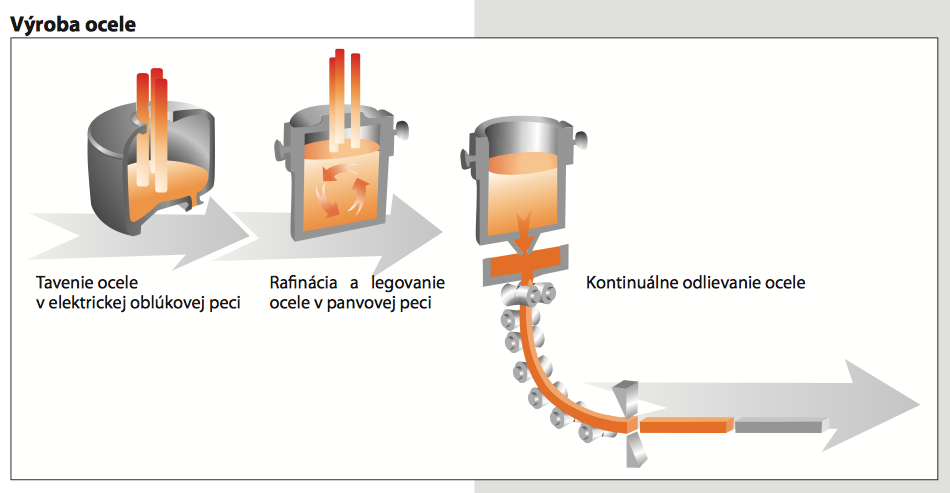
\includegraphics[width=\textwidth]{vyroba_ocele.png}
	\caption{Proces výroby ocele}
\end{figure}

\begin{figure}[h!]
	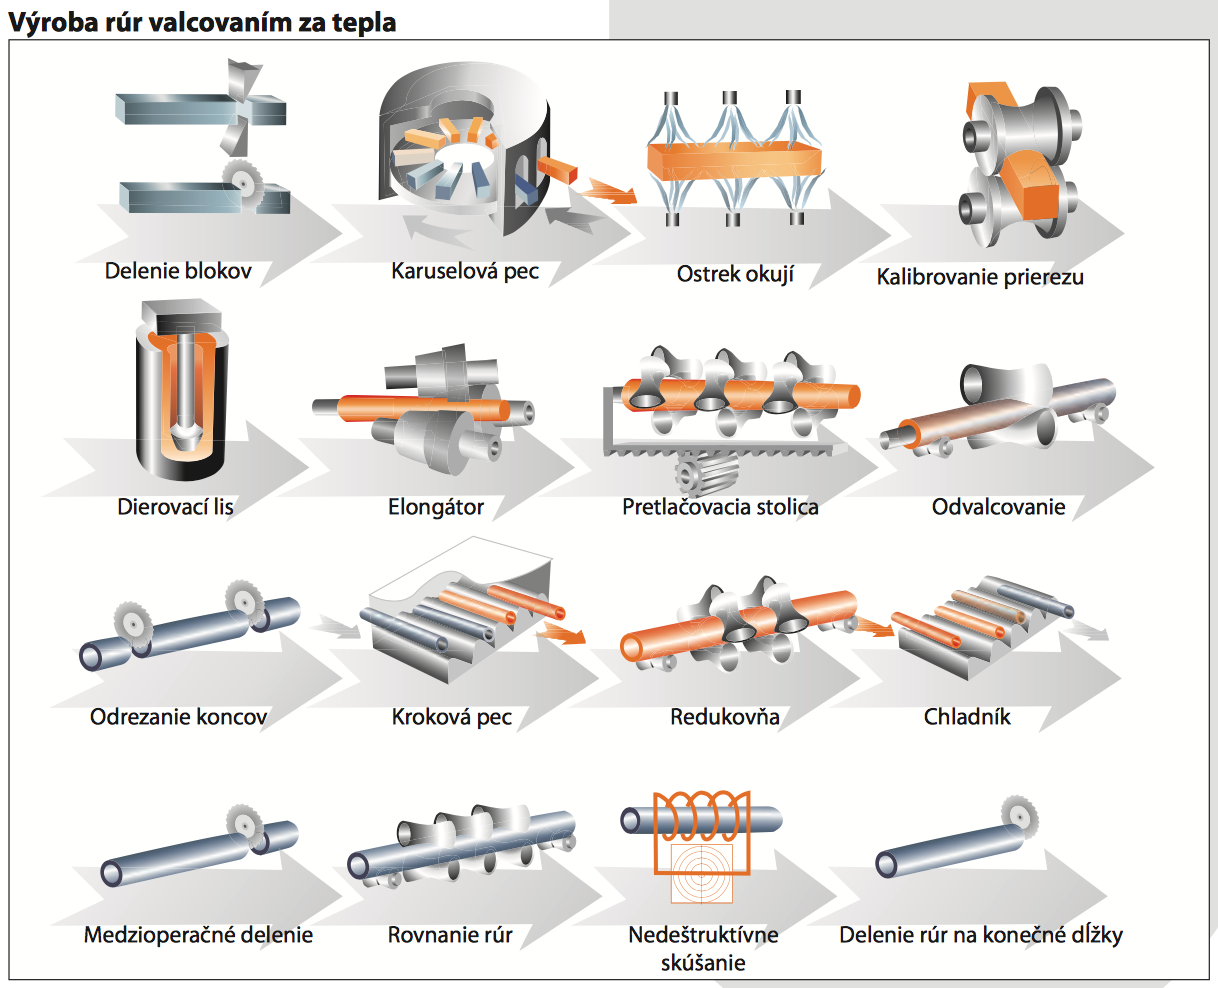
\includegraphics[width=\textwidth]{vyroba_rur.png}
	\caption{Proces výroby rúr}
\end{figure}

\newpage

\begin{figure}[h!]
	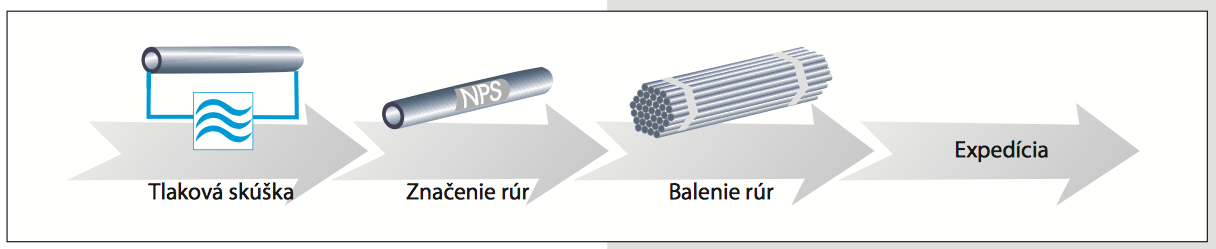
\includegraphics[width=\textwidth]{expedicia.png}
	\caption{Finálne skúšky, balenie, expedícia}
\end{figure}

Výrobný proces rúr je modelovaný ako SHO\footnote{\url{https://www.fit.vutbr.cz/study/courses/IMS/public/prednasky/IMS.pdf}, strana 136} a je popísaný formou Petriho siete\footnote{\url{https://www.fit.vutbr.cz/study/courses/IMS/public/prednasky/IMS.pdf}, strana 123}.

\begin{figure}[h!]
	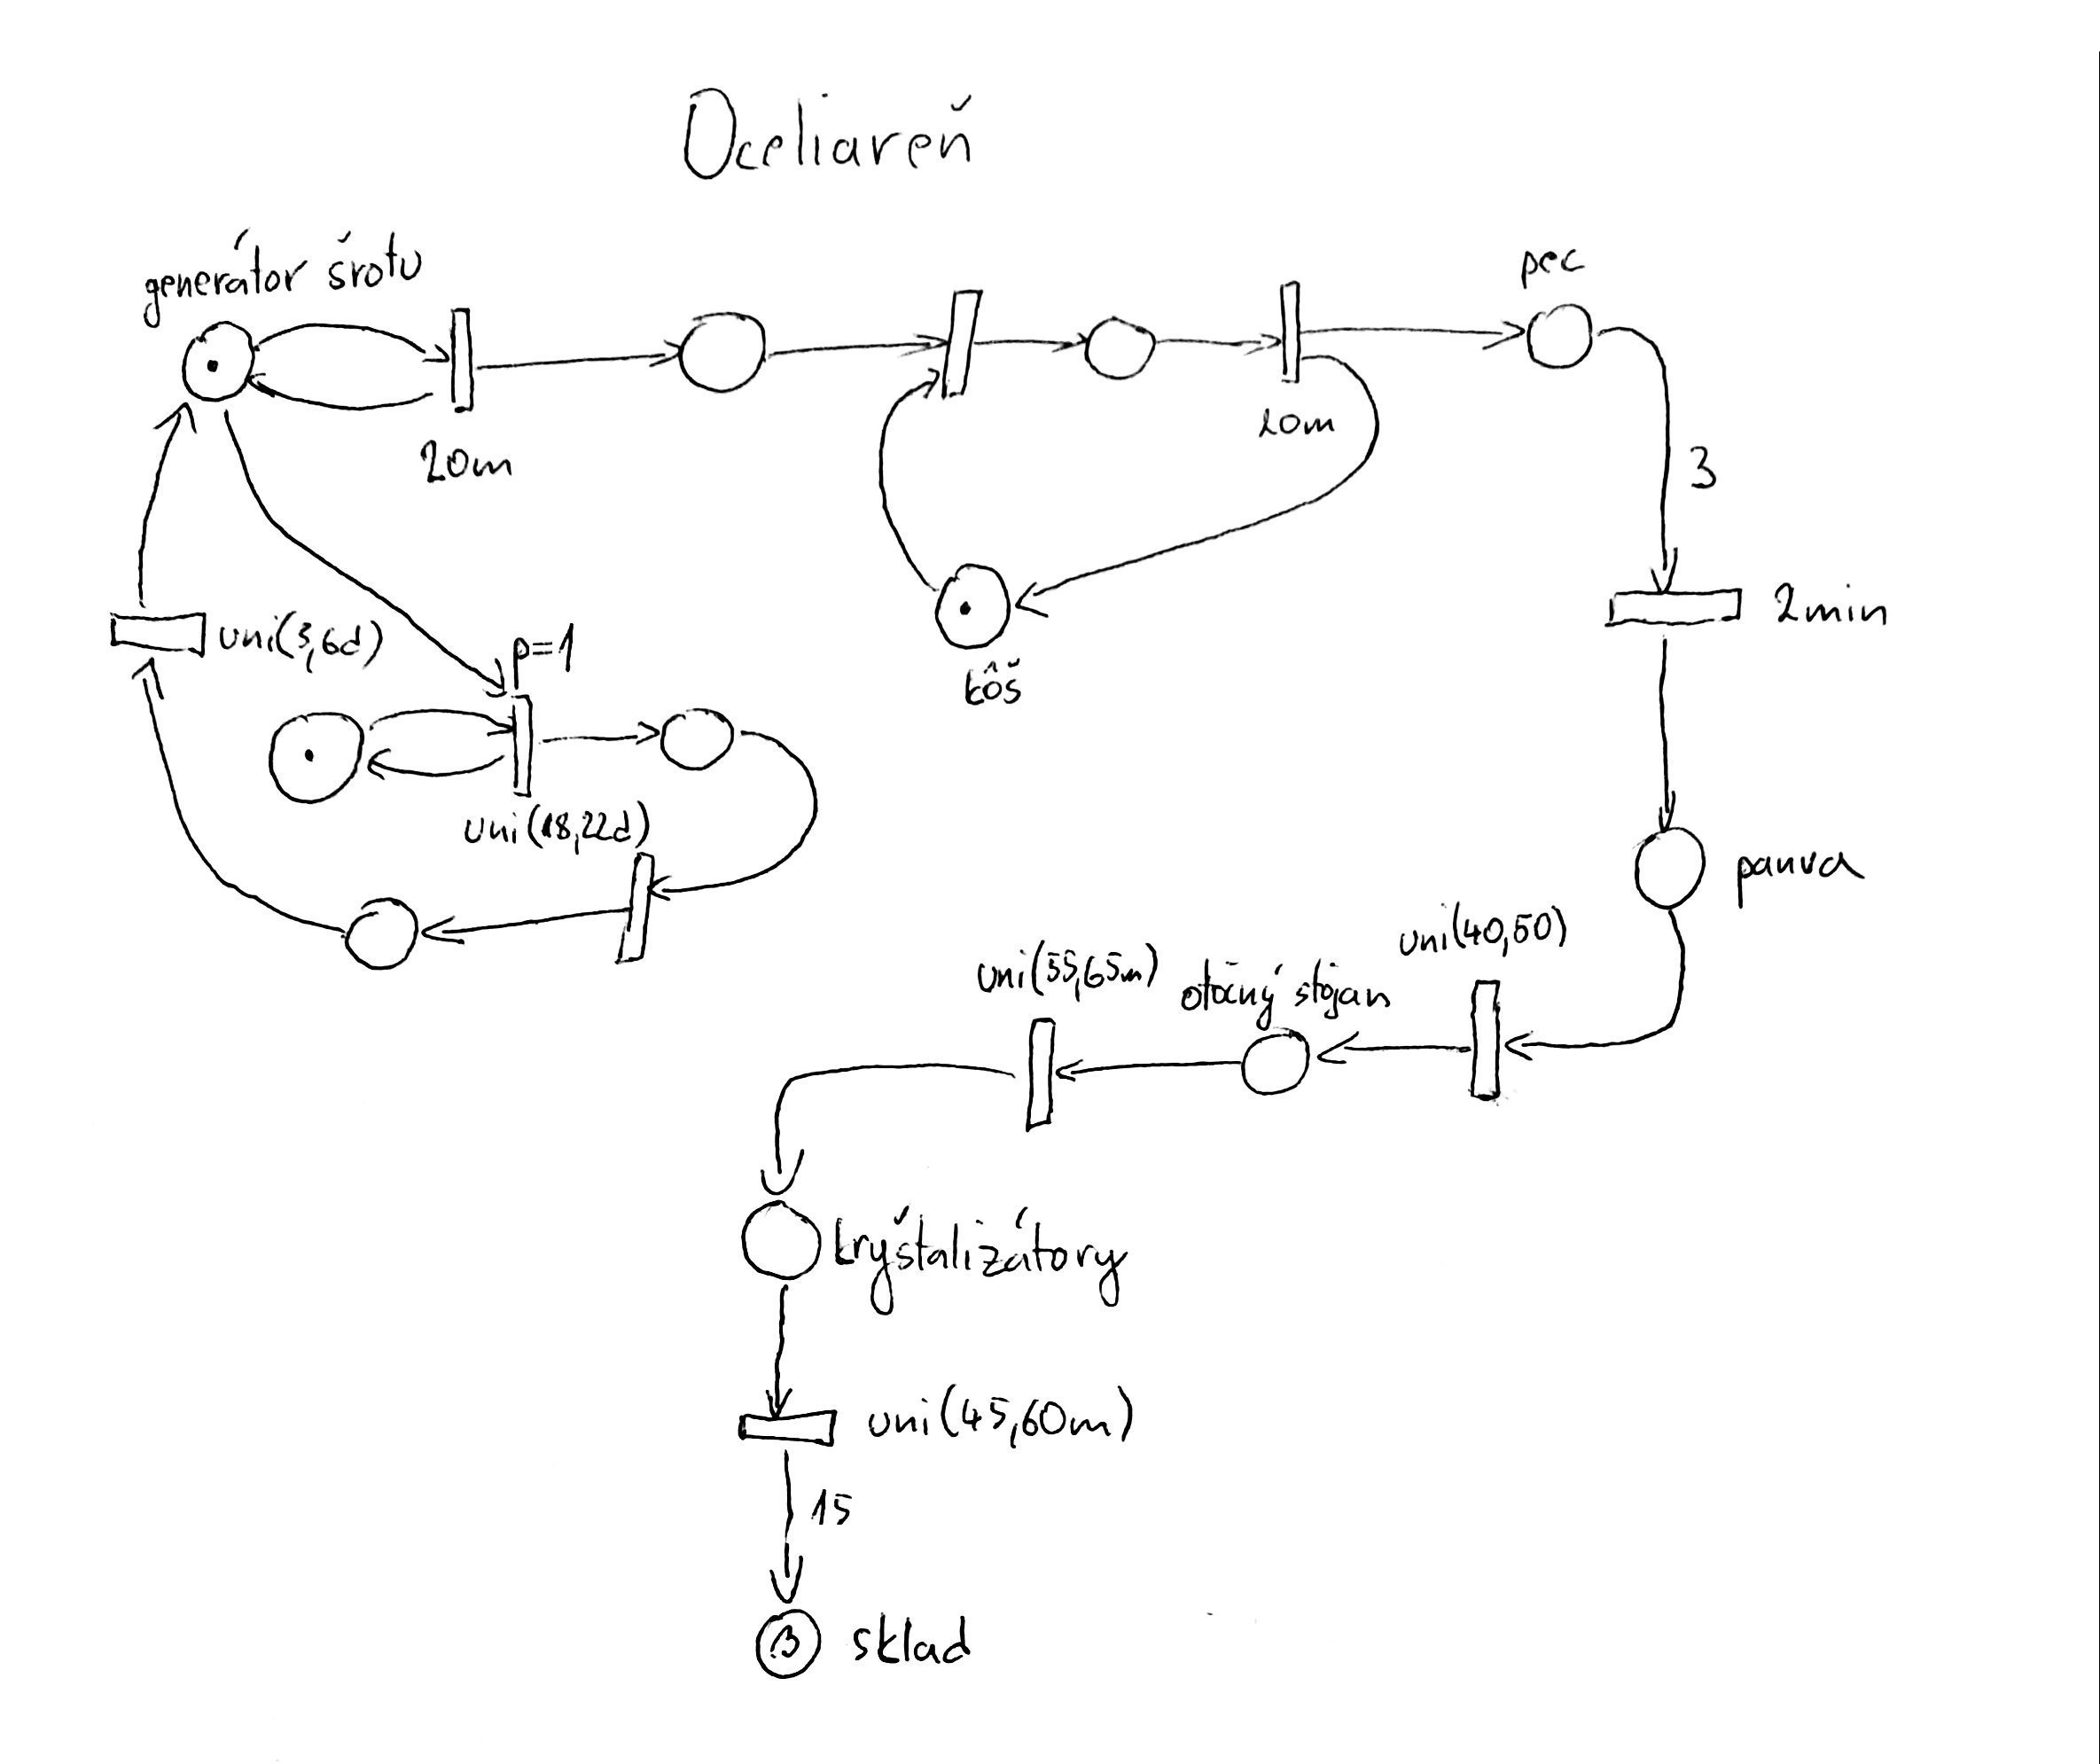
\includegraphics[width=\textwidth]{pn_oceliaren.jpg}
	\caption{Petriho sieť pre oceliareň}
\end{figure}

\begin{figure}[h!]
	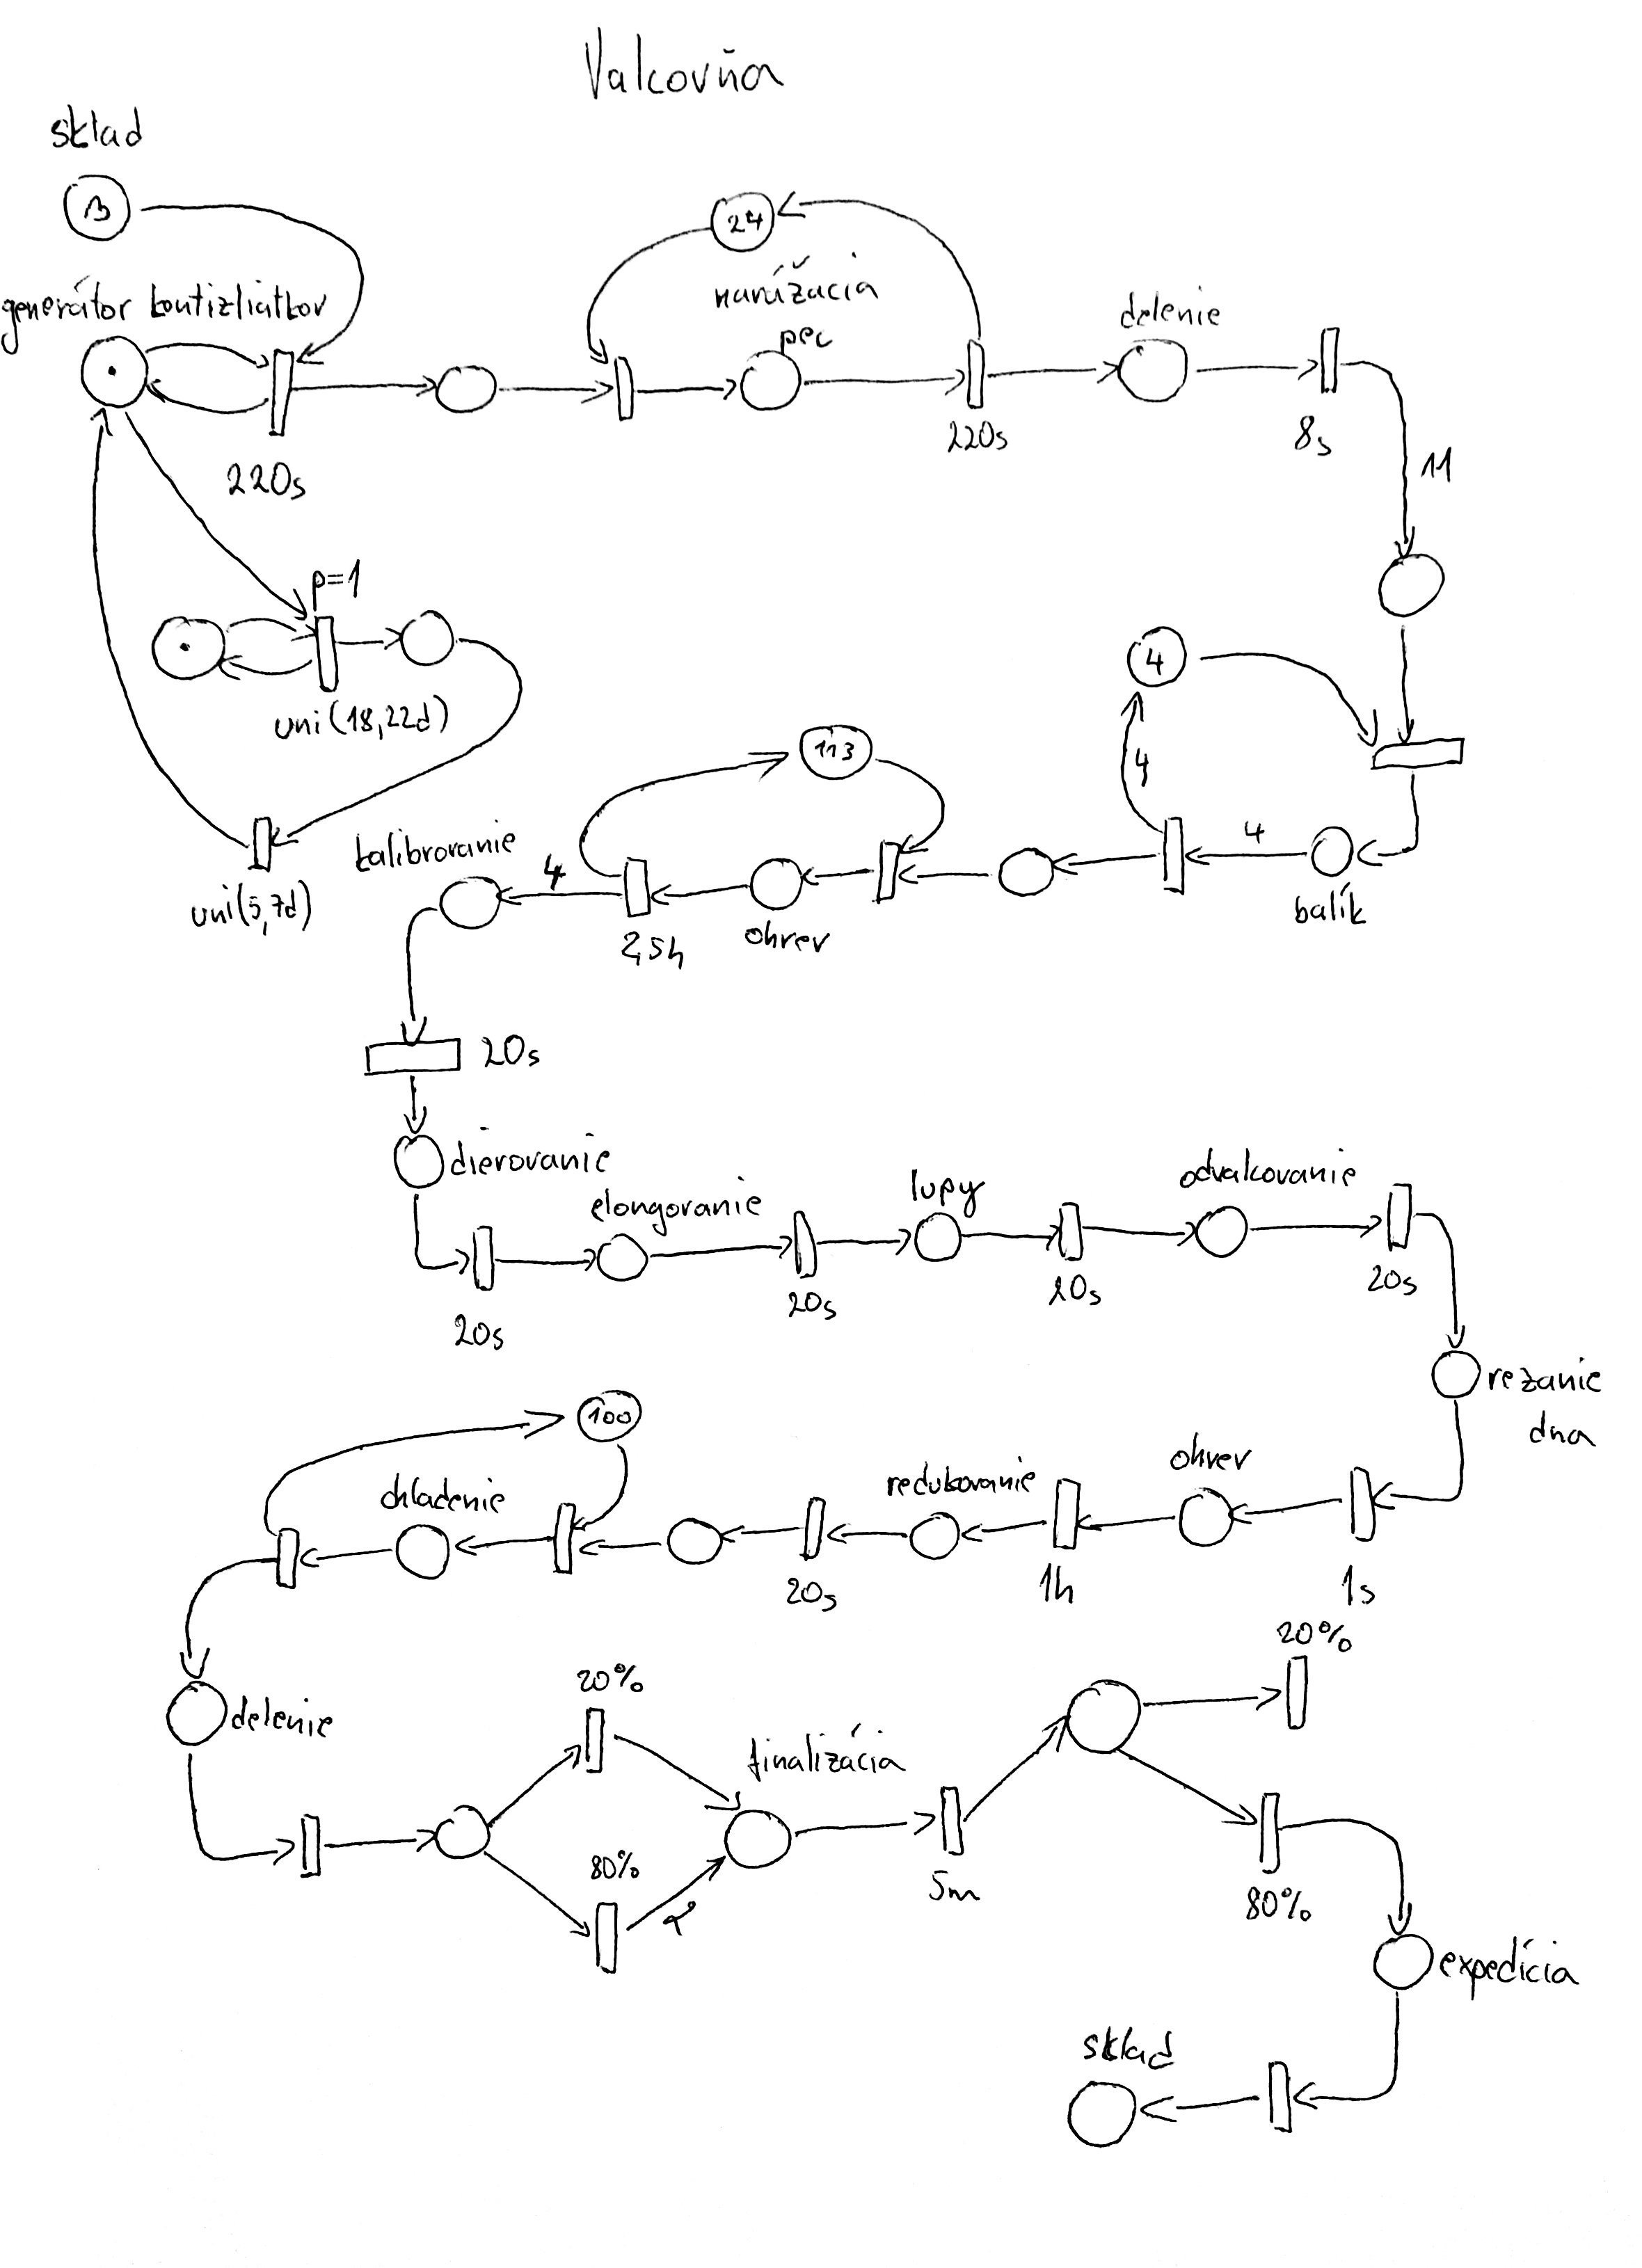
\includegraphics[width=\textwidth]{pn_valcovna.jpg}
	\caption{Petriho sieť pre valcovňu}
\end{figure}

\newpage
	
\subsection{Formy konceptuálneho modelu}
V~našom simulačnom modeli nezohľadňujeme šrotové pole, pretože z~pohľadu toho čo skúmame je to nepodstatné. Predpokladáme, že šrotu je stále dosť a vždy keď ho systém potrebuje ho má k~dispozícii. Systém oceliarne začína príchodom šrotu vo vsádzkových košoch. Tie chodia do pece každých 15 minút. Avšak, taviaci modul pracuje v~dvoch fázach, pričom v~druhej sa šrot už nepridáva. Roztavenie jednej vsádzky trvá hodinu. My sme si túto realitu zabstrahovali tak, že druhú fázu vynecháme, no zároveň predĺžime príchod vsádzkových košov na dvadsať minút. Pec taví priebežne, čo máme modelované ako stav, v~ktorom sa čaká na 60 ton ktoré do pece prídu. Keďže vsádzkový kôš má kapacitu 20 ton, a chodí každých 20 minút, získame tým požadovaný výkon pece 60 ton za hodinu.

Z~pece sa do panvy odpichuje 54.5 ton. To sme zlúčili do jedného balíka päťdesiatich-štyroch ton roztavenej ocele. V~oceliarni s~tým budeme pracovať ako s~jednou transakciou. Odpich trvá 2 minúty.
V~panvovej peci sa roztavená oceľ dodatočne spracováva, čo trvá v~priemere 45 minút (záleží na akosti). Preto sme sa rozhodli tento prechod modelovať ako rovnomerné rozloženie pravdepodobnosti medzi štyridsiatimi a päťdesiatimi minútami.

Prevoz medzi panvovou pecou a zariadením plynulého odlievania trvá v~priemere 10 minút. Záleží od toho, v~akom stave sú stroje, ako rýchlo sa panvu podarí uchopiť a akou rýchlosťou sa panva preváža. Preto sme sa rozhodli v~tomto stave zvoliť rovnomerné rozloženie pravdepodobnosti medzi ôsmimi a dvanástimi minútami.

Odlievanie trvá priemerne 60 minút, no keďže balík roztavenej ocele môže trochu kolísať, (záleží aký šrot sa tam hodí na spracovanie), rozhodli sme sa pre rovnomerné rozloženie pravdepodobnosti odlievania medzi 55 a 65 minútami.

Následne sú kontizliatky vychladené. To vo firme trvá 45 až 60 minút, čo sme sa rozhodli zachovať. Preto náš prechod pri chladení má taktiež rovnomerné rozloženie pravdepodobnosti medzi 45 a 60 minútami.

Výrobok oceliarne sa za istý čas dopraví do medzioperačného skladu. Preprava avšak nehrá v~systéme žiadnu rolu. Najme kvôli tomu, že v~sklade majú nejaké zásoby a valcovňa nemusí čakať na to, kým sa z~chladníka privezú na sklad kontizliatky. Preto sme sa tento čas rozhodli zanedbať. Pri produkcii oceliarne a nastavených požiadavkách valcovne sa kontizliatky vyrábajú rýchlejšie. V~priemere 30 \% kontizliatkov sa predáva externým zákazníkom. Preto nepridávame do skladu 21 kontizliatkov z~jednej tavby ale 15.

Oceliareň vyrába 81 \% času a teda z~každých 20 dní v~roku v~priemere 4 nevyrába. Preto s~rovnomerným rozložením pravdepodobnosti medzi 18 až 22 dní sa stane prerušenie výroby s~rovnomerným rozdelením pravdepodobnosti medzi 3 až 6 dňami.

Z~medzioperačného chodia do systému valcovne kontizliatky každých 220  sekúnd. Tie putujú do narážacej pece, v~ktorej ostávajú hodinu. Po hodine sa z~nej jeden za druhým vyberajú. Z~pohľadu modelu to vyzerá tak, že prvú hodinu sa z~narážacej pece nič neprodukuje a potom každých 220 sekúnd jeden kontizliatok. Túto časť systému sme sa snažili zabstrahovať kvôli náročnosti výpočtov. Zanedbávame prvú hodinu a rovno modelujeme, že kontizliatok je v~peci 220 sekúnd a ide z~nej preč spracovaný. Z~dlhodobého hľadiska nerobí táto abstrakcia žiadny alebo len minimálny rozdiel.

Kontizliatky sa následne delia na menšie, čo trvá v~priemere 8 sekúnd. Výsledkom je 11 menších blokov určených na ohrev. Preto pri delení máme na tvrdo osem sekúnd a neriešime nejaké rozloženie pravdepodobnosti. Osem sekúnd je z~hľadiska celého systému zanedbateľná hodnota.
Nasleduje karuselová pec, ktorá má kapacitu 113-tich krokov po štyroch malých blokoch. Tu sme použili abstrakciu, v~ktorej sme zväzok štyroch blokov dali do jedného celku. Balík zotrváva v~karuselovej peci 2.5 hodiny.

Abstrakcia použitá pri karuselovej peci sa ďalej už používať nemôže, z~dôvodu, že ďalej v~systéme pracujeme s~každým blokom osobitne. Nasleduje kalibrácia, ktorá má rýchlosť 3.6 kusa za minútu. Keďže je fabrika nastavená na tri bloky za minútu, vychádza to 20 sekúnd na jeden kus. Za tým ide dierovanie, v~ktorom to je podobne, spracovanie elongátorom a výber lupy. Všetky tieto moduly sú optimalizované na 20 sekúnd na jeden blok.

Nasleduje odvalcovacia stolica, ktorá má výkon 1.38 metra odvalcovanej rúry za sekundu. V~našom systéme počítame s~priemernou dĺžkou rúry, ktorá je 35 metrov. Jednoduchým výpočtom zistíme, že odvalcovanie jednej rúry trvá približne 20 sekúnd. Z~hľadiska celého systému je táto hodnota zanedbateľná a teda ju tam máme na tvrdo, bez žiadneho pravdepodobnostného rozloženia.
Nasleduje rezanie dna pílou, ktorá je schopná spracovať 100 metrov za sekundu. Pri našom výpočte 35 metrových rúr rátame s~prechodom kde sa čaká jednu sekundu.

Po odrezaní dna nasleduje ohrev a redukcia ktoré sa riadia rýchlosťou 3.4 kusov za minútu, čo dáva prechod 20 sekúnd na jednu rúru. Rúry su v~peci hodinu.

Keď sú rúry zredukované, putujú do krokového chladníka. Pri kadencii rúr na chladník, ktorá je 3.4 kusov za minútu na 100 krokoch chladníka trvá chladenie v~priemere  po zaokrúhlení 30 minút. Preto sme sa to rozhodli modelovať ako rovnomerné rozloženie pravdepodobnosti medzi 25 až 35 minút.
Delenie násobných dĺžok sa nerobí vždy, pretože rúry môžu mať dĺžku aj pod 21 metrov. I~napriek tomu, že rátame s~priemerom 35 metrov tento jav zohľadňujeme. V~20 \% prípadov sa rúra deliť nemusí a v~80 \% áno.
Po delení násobných dĺžok prebieha finalizácia, ktorá trvá 5 minút a nakoniec expedícia. V~našom modeli nezohľadňujeme počas celého procesu odpad (orezávanie koncov, vyhodenie pri kontrolách...). Túto skutočnosť zohľadňujeme pred expedíciou, kde 20 \% produktov automaticky vyhadzujeme.
Valcovňa vyrába 70 \% času a teda každých 20 dní v~roku sa priemerne 6 dní nevyrába. Preto s~rovnomerným rozložením pravdepodobnosti medzi 18 až 22 dní sa stane prerušenie výroby s~rovnomerným rozdelením pravdepodobnosti medzi 5 až 7 dňami.


\section{Architektúra simulačného modelu}
Ako sme už spomenuli v~kapitole 2.2, implementácia simulačného modelu je v~jazyku C++ a využíva knižnicu SIMLIB. Simulačný model využíva prvky objektovo-orientovaného programovania.

\subsection{Mapovanie konceptuálneho modelu na simulačný}
Jednotlivé triedy v~simulačnom modeli popisujú entity v~konceptuálnom modeli.

\begin{center}
	\begin{table}[!h]
		\centering
		\begin{tabular}{|c|c|} 
			\hline
			entita v~konceptuálnom modele & trieda v~simulačnom modeli \\
			\hline
			\hline
			príchody šrotu & GeneratorDavkySrotu \\
			\hline
			príchody kontizliatkov & GeneratorKontizliatkov \\
			\hline
			prichádzajúce prerušenia v~oceliarni & GeneratorPreruseniaVOcielarni \\
			\hline
			prichádzajúce prerušenia vo valcovni & GeneratorPreruseniaVOValcovni \\
			\hline
			prvotné naplnenie skladu & NaplnenieSkladu\\
			\hline
			príchody šrotu & GeneratorDavkySrotu \\
			\hline
			hmota ocele určená na odpich & PracovnaHmota \\
			\hline
			kontizliatok (medzivýrobok z~oceliarne) & Kontizliatok \\
			\hline
			časť kontizliatku po rozstrihaní & Blok \\
			\hline
			štyri bloky určené na ohrev & OhrevnyBalik \\
			\hline
			blok po ohreve v~karuselovej peci & OhriatyBlok \\
			\hline
			hotová rúra určená na expedíciu & Rura \\
			\hline
		\end{tabular}
		\caption{Mapovanie konceptuálneho modelu na simulačný model}
	\end{table}
\end{center}

\section{Podstata experimentov a ich priebeh}
Cieľom experimentov bolo zistiť, ktoré vlastnosti systému ako ovplyvňujú výrobu, a čo je pre firmu viac alebo menej výhodné. Sledovať, na aký sortiment sa majú zamerať, prípadne ako veľmi sa snažiť znížiť prestoje. Zároveň budeme experimentovať s~kadenciou blokov putujúcich cez valcovňu.

\subsection{Postup experimentovania}
Po tom, čo sme si overili, že informácie sedia na priemerných hodnotách systému sme začali prepočítavať rôzne vstupy. Upravovali sme veľkosti blokov, čím sa nám menil počet narezaných blokov z~jedného kontizliatku a kadencia kontizliatkov do valcovne. Potom sme sa zamerali na znižovanie prestojov a na záver sme upravili kadenciu na najvyššiu možnú. Spustili sme model päť až desať krát a spravili priemer.

\subsection{Dokumentácia jednotlivých experimentov}
Vykonali sme niekoľko experimentov za účelom získania nových znalostí o~modelovanom systéme.

\subsubsection{Zmena veľkosti blokov}
Najskôr sme zmenili priemerný blok na jeden meter. Sortiment rúr sa tým zmenil na väčšie rúry. Počet kusov z~jedného 8 metrového kontizliatku je 8, čím sa kadencia kontizliatkov do valcovne znížila na dve minúty aj štyridsať sekúnd. Zároveň sme museli upraviť expedíciu v~oceliarni. Pri takomto sortimente sme museli všetky kontizliatky dávať do skladu a žiadne neexpedovať externým firmám. Priemerná ročná produkcia pri takomto sortimente sa zvýšila o~zhruba 40 \% na 280 000 ton.

V~ďalšom experimente sme zmenili priemernú dĺžku bloku na pól metra. Sortiment rúr sa zmenil na menšie rúry a počet kusov z~jedného 8 metrového kontizliatku na 16. Kadencia kontizliatkov do valcovne sa teda zvýšila na 5:20 minút. Ročná produkcia sa znížila o~29 \% na 142 000 ton. Zároveň ale nám oceliareň produkovala viac kontizliatkov ako sme vo valcovni potrebovali a teda sme ich mohli predávať externým zákazníkom.

\subsubsection{Zmena prestojov na prevádzkach}
Ako prvú sme si zobrali oceliareň. Prestoje sú započítané v~poruchách a dokopy to je za rok 13 \% celkového času. Po zmenšení prestojov o~3 percentá sme dostali väčší výkon oceliarne o~2.2 \%. Zvýšil sa v~priemere na 378 000 ton ročne.

Ak zmenšíme prestoje ešte o~ďalšie 2 percentá, dostaneme výkon oceliarne väčší o~4.1 \% na približne 385 000 ton ročne.

Po znížení prestojov na valcovni o~2 percentá sa produkcia valcovne zvýšila na približne 5 \% na 210 000 ton ročne.

\subsubsection{Zmena kadencie blokov vo valcovni}
Kadencia vo valcovni sa môže meniť v~rámci najpomalšieho prvku výroby. Preto sme mohli kadenciu zvýšiť na maximálne 3.4 kusu za minútu. Pri zachovaní priemernej dĺžky bloku na 0.72 metra, sa priemerný výkon valcovne zvýši o~7 \%, čo je z~200 000 ton na 214 000 ton valcovaných rúr ročne.

\newpage

\subsubsection{Závislosť medzi dobou príchodov šrotu do oceliarne na výrobu}
V~tomto experimente sme menili časový interval medzi príchodmi šrotu (dávok šrotu -- 20 ton) a sledovali vplyv tejto zmeny na výrobu kontizliatkov a samotných rúr. Sledované obdobie bol jeden rok.

Nasledujúce grafy prezentujú získané výsledky z~experimentovania.
\begin{figure}[h!]
	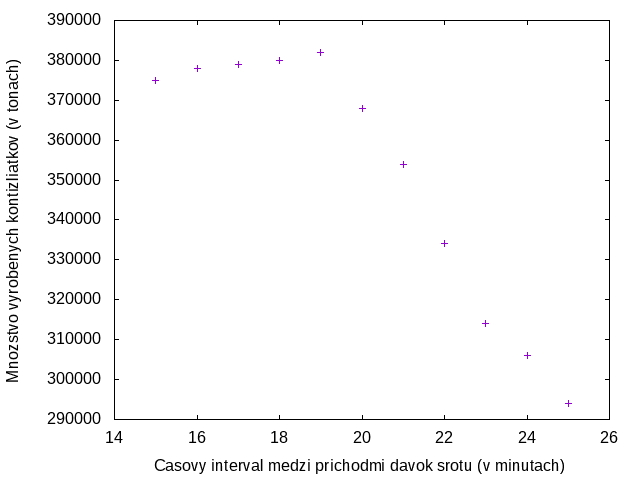
\includegraphics[width=\textwidth]{prichody_srotu_konti.png}
	\caption{Závislosť medzi dobou príchodov šrotu do oceliarne na celkovú výrobu kontizliatkov}
\end{figure}

Ako je možné vidieť z~grafu, hodnota 20 minút je hraničná, od tejto hodnoty už dochádza ku klesaniu výroby kontizliatkov.

\begin{figure}[h!]
	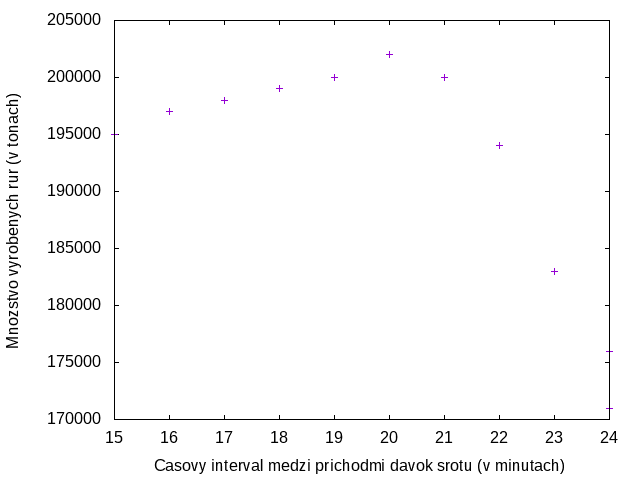
\includegraphics[width=\textwidth]{prichody_srotu_rury.png}
	\caption{Závislosť medzi dobou príchodov šrotu do oceliarne na celkovú výrobu rúr]}
\end{figure}

Experiment poukazuje na fakt, že skorší príchod o~minútu-dve je takmer zanedbateľný na celkovú výrobu rúr, no oneskorenie sa o~vyše minútu (interval príchodov väčší ako 21 minút) znamená znateľný pokles výroby. Preto je dôležité priebežne kontrolovať túto dobu, či nejaká na prvý pohľad zanedbateľná zmena v~príchod dávok šrotu nespôsobí viac ako minútové oneskorenie, čo, ako sme experimentálne zistili, ma značný dopad na výrobu.

Graf taktiež ukazuje, že k~najefektívnejšej výrobe dochádza pri hodnotách príchodov šrotu 19, 20 a 21 minút. Na tieto hodnoty sme sa zamerali detailnejšie, s~ohľadom aj na využitie skladu kontiklatikov. Vykonali sme ďalšie experimenty, skúmajúce stav skladu (na začiatok sme naplnili sklad kontizliatkami na polovicu jeho kapacity, t.j. 5000) pri intervaloch príchodu šrotu zo skúmanej množiny, t.j. \{19, 20, 21\}.

\begin{center}
	\begin{table}[!h]
		\centering
		\begin{tabular}{|c|c|c|c|} 
			\hline
			interval & minimálne využitie & maximálne využitie & priemerné využitie\\
			\hline
			\hline
			19 minút & 4999 & 10000 & 7828 \\
			\hline
			20 minút & 4499 & 7093 & 8977 \\
			\hline
			21 minút & 963 & 5792 & 4183 \\
			\hline
		\end{tabular}
		\caption{Stavy na sklade pri rôznych intervaloch príchodu šrotu}
	\end{table}
\end{center}

Z~výsledkov experimentu vyplýva, že pri intervale príchodov šrotu 19 minút dochádza k~tomu, že sklad nestíha výrobe, výroba kontizliatkov je prirýchla a je rýchlo dosiahnutá jeho maximálna kapacita, čo je neželaný stav. 

Pri hodnote 20 minút je sklad využívaný efektívne, stíha výrobe, nedochádza k~tomu, žeby bola dosiahnutá jeho maximálna kapacita. Ide teda o~vhodný interval príchodu šrotu.

Pri intervale 21 minút dochádza k~tomu, že výroba je pomalá, v~sklade je často dosť málo kontizliatkov a je tu riziko že sa vyprázdni a valcovňa by v~takom prípade stála a čakala, čo je tiež neželaný stav.

\subsubsection{Závislosť medzi dobou príchodov kontizliatkov na výrobu rúr}
V~tomto experimente sme menili časový interval medzi príchodmi kontizliatkov a sledovali vplyv tejto zmeny na výrobu rúr. Sledované obdobie bol jeden rok.

\begin{figure}[h!]
	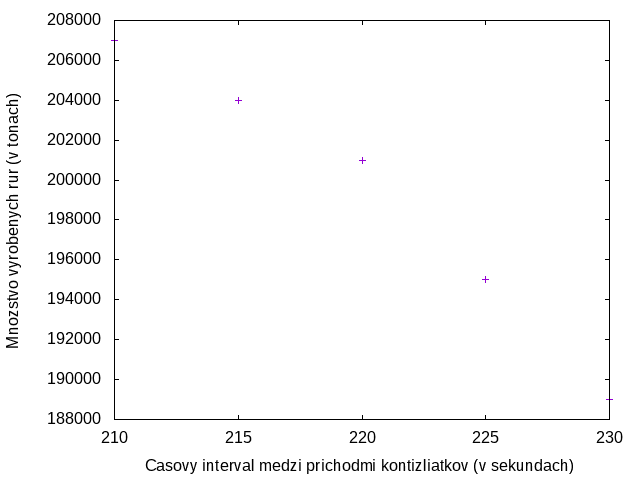
\includegraphics[width=\textwidth]{prichody_konti_rury.png}
	\caption{Závislosť medzi dobou príchodov kontizliatkov na celkovú výrobu rúr}
\end{figure}

Graf ukazuje, že čím nižší je interval príchodov kontizliatkov, tým sa výroba zvyšuje. No taktiež je ale potrebné do úvahy brať technické obmedzenia strojov, že jedna výrobná fáza sa nemôže príliš zrýchliť (interval pod hranicou 215 sekúnd) lebo je to technicky nezrealizovateľné, stroje by nestíhali. Pársekundová zmena by však mohla byť technicky realizovateľná. Ako je vidno z~grafu, zmena na interval 215 sekúnd znamená pre ročnú výrobu nárast o~vyše 2 000 ton. 

\subsubsection{Závery experimentov}
Základné experimenty sa týkali zisťovania výroby za jednotku času (1 rok) a pomáhali nám pri ladení samotného modelu, aby bol čo možno najviac podobný skutočnému systému.

Na základe ďalších experimentov môžeme povedať, že zmena sortimentu má na výslednú produkciu valcovne najväčší vplyv. Zároveň je ale menej kontizliatkov na predaj externým zákazníkom. Zmeny prestojov dlhodobo ovplyvnia len pár percent, no i to sa dá považovať ako za dostatočnú zmenu. Pri zvyšovaní kadencie nastáva problém, pri fyzických schopnostiach daných strojov. To že sú nakalibrované na vyššie je skôr rezerva. V~reálnom systéme sa stáva, že nejaký blok sa spozdí o~pár desatín sekundy a to by mohlo pri maximálnej kadencii spôsobiť poruchu a poškodenie systému. Experimentom sme taktiež preskúmali intervaly príchodu šrotu a následne ich dopad na celkovú výrobu. Získané výsledky hovoria o~tom, že najoptimálnejšia doba príchodu šrotu je 20 minút. V~prípade nižšej už dochádza dosiahnutiu kapacitných možností skladu. V~prípade vyššej hrozí, že v~sklade nebude dostatok kontizliatkov a valcovňa bude čakať. Oneskorenie o~vyše minútu u~príchodu šrotu do valcovne taktiež znamená znateľné zníženie celkovej výroby.

\section{Shrnutie simulačných experimentov a záver}
Z~výsledkov experimentov vyplýva, že typ sortimentu má na výslednú produkciu najväčší dopad. Samotné prestoje a ich prípadne zmeny v~dlhodobom rozsahu ovplyvnia len mierne, no ale i tak hovoríme v~prípade roka o~zmenu o~rozmedzí niekoľko tisíc ton. Pri zvýšenej kadencii sa výroba podľa experimentu značne zvyšuje, no obmedzením sú samotné stroje a ich technické možnosti. Pársekundová zmena by však mohli byť technicky realizovateľná, no závisí ďalej aj o~ďalších faktov, ako by sa zvýšilo opotrebovanie strojov a ich kazivosť. Je taktiež potrebné pri výrobe dôkladne kontrolovať a dodržiavať interval príchodov šrotu -- experiment poukázal na fakt, že zmena intervalu čo i len o~minútu spôsoby problémy so skladom. Ďalej, oneskorenie len o~vyše minútu znamená znateľné zníženie celkovej výroby (prepad v~ročnej výrobe o~6 000 ton).

V~rámci projektu vznikol nástroj na simuláciu výrobného procesu v~železiarni, pokrývajúci oceliareň a valcovňu. Vychádza z~údajov, ktoré sme získali konzultáciami s~vedúcim výroby v~železiarni. Program reprezentujúci simulačný model bol implementovaný v~jazyku C++ a na jeho tvorbu bola použitá knižnica SIMLIB.

\end{document}